
\documentclass[10pt]{beamer}

\usetheme{metropolis}
\usepackage{appendixnumberbeamer}
\usepackage{graphicx}
\usepackage{animate}
\usepackage{hyperref}
\usepackage{booktabs}
\usepackage[scale=2]{ccicons}
\usepackage{tikz}
\usetikzlibrary{positioning}
\usepackage{pgfplots}
\usepgfplotslibrary{dateplot}
\usepackage{subcaption}
\usepackage{xspace}
\newcommand{\themename}{\textbf{\textsc{metropolis}}\xspace}
\title{Low-level controller for non-holonomic omnidirectional mobile robot}
\date{\today}
\author{Lingyuan Yang}
\institute{Technische Universität Berlin\\ABB Corporate Research}


\tikzset{
    wheelFrame/.pic={
		\draw[gray, very thick] (-0.8,-0.1) rectangle (0.8,0.1);
		\filldraw [gray] (0,0) circle (1pt);
		\draw[->] (0,0) -- (1,0) node[anchor=north west] {$x^{w#1}$};
		\draw[->] (0,0) -- (0,1) node[anchor=north west] {$y^{w#1}$}; 
	}
}
\tikzset{
    wheel/.pic={
		\draw[gray, very thick] (-0.8,-0.1) rectangle (0.8,0.1);
		\filldraw [gray] (0,0) circle (1pt);
	}
}


\tikzset{
    platform/.pic={
		\filldraw [gray] (0,0) circle (2pt);
			\draw[thick,->] (0,0) -- (5,0) node[anchor=north west] {$x^b$};
			\draw[thick,->] (0,0) -- (0,5) node[anchor=south east] {$y^b$};
			\draw[thick,->] (0.75,0) arc (0:90:0.75) node[anchor=south west] {$\theta^b$};
			\draw[black, thick] (-3,-3) rectangle (3,3);
	}
}










\begin{document}

\maketitle

\begin{frame}{Table of contents}
  \setbeamertemplate{section in toc}[sections numbered]
  \tableofcontents[hideallsubsections]
\end{frame}

\section{Introduction}
%%%%%%%%%%%%%%%%%%%%%%%%%%%%%%%%%%%%%%%%%%%%%%%%%%%%%%%%%%%%%%%%%
\begin{frame}{Mobile Platform}
    \begin{figure}
        \centering
        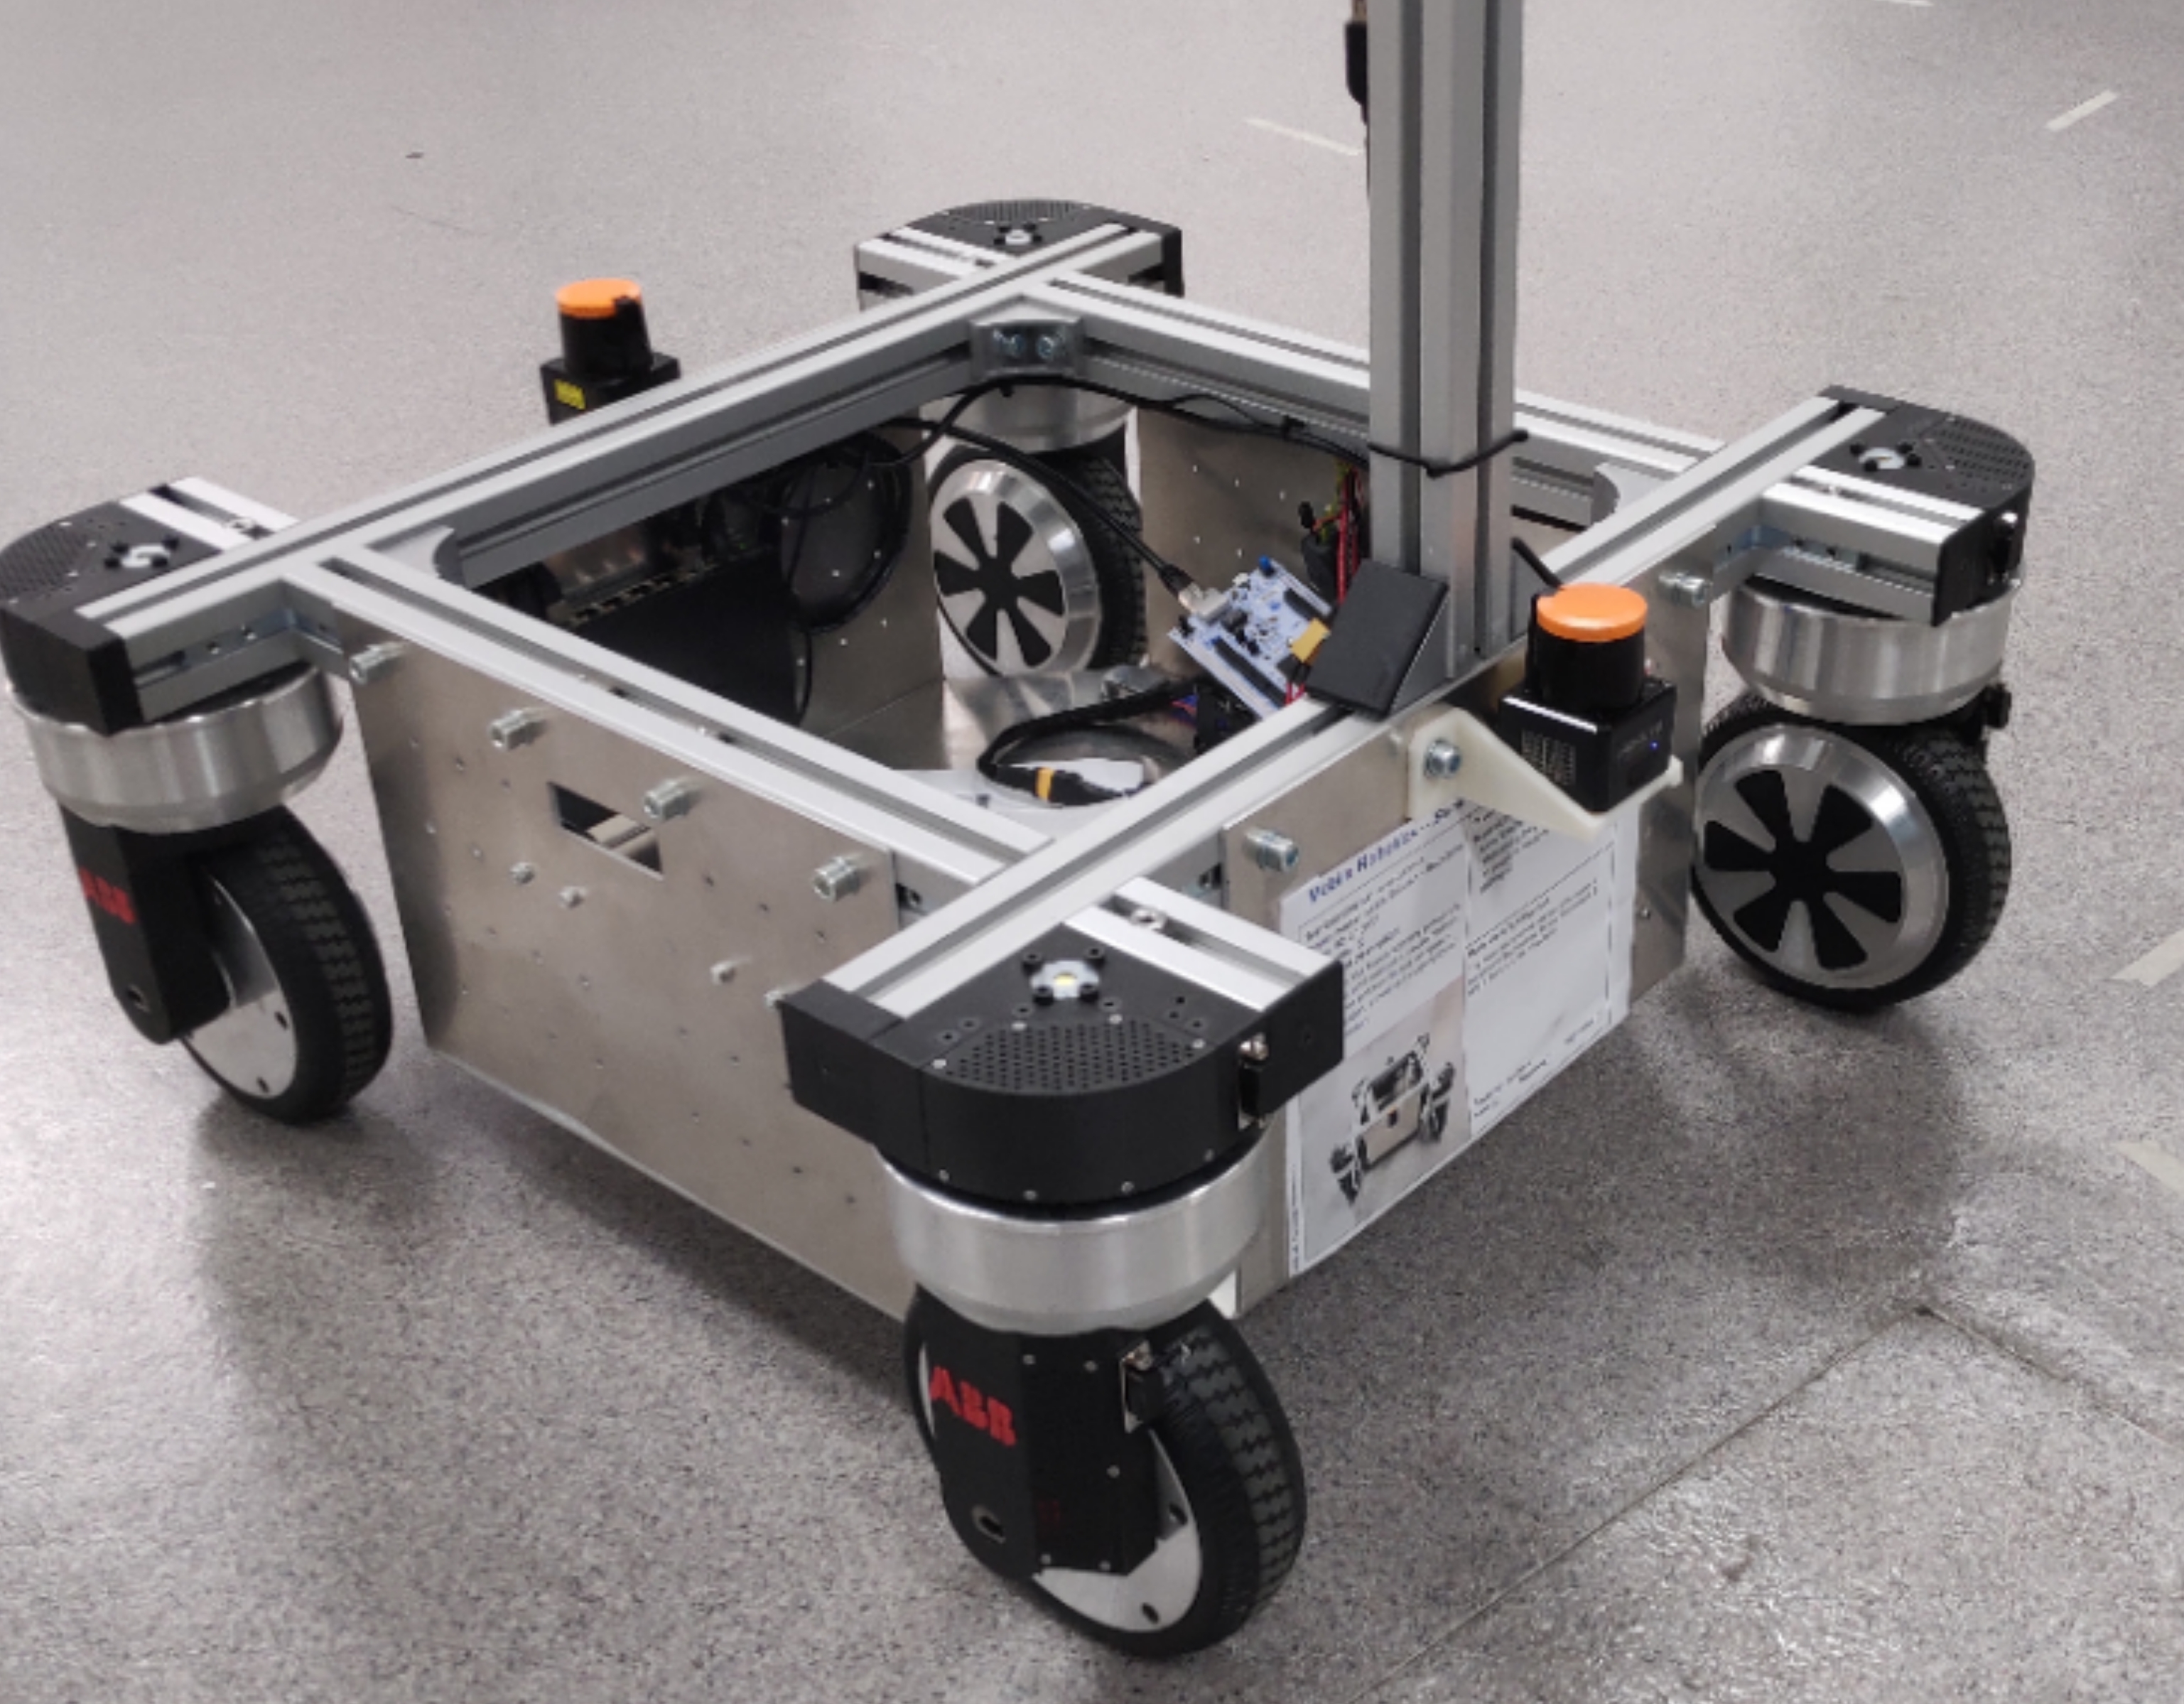
\includegraphics[width=\textwidth]{Figure/mobilePlatform.jpg}
        \caption{}
        \label{fig:mobilePlatform}
    \end{figure}
\end{frame}
%%%%%%%%%%%%%%%%%%%%%%%%%%%%%%%%%%%%%%%%%%%%%%%%%%%%%%%%%%%%%%%%%
\begin{frame}{Non-holonomic omnidirectional mobile robot}
    	\begin{alertblock}{Non-holonomic}
		\textbf{Controlable DoF less than DoF} The mobile robot have 3 DoF $x,y,\theta$. But it cannot do arbitrary velocity instantaneously. The wheels needs to orient to a certain position to achieve a certain velocity. Eg. move sideways.
	\end{alertblock}
\end{frame}
%%%%%%%%%%%%%%%%%%%%%%%%%%%%%%%%%%%%%%%%%%%%%%%%%%%%%%%%%%%%%%%%%
\begin{frame}{Non-holonomic omnidirectional mobile robot}
    	\begin{alertblock}{omnidirectional}
		The mobile robot can acheive any task space velocity $\dot{x},\dot{y},\dot{\theta}$ if properly initialized.
		Eg. turn all the wheels 90 degree to move sideways.
	\end{alertblock}
\end{frame}
%%%%%%%%%%%%%%%%%%%%%%%%%%%%%%%%%%%%%%%%%%%%%%%%%%%%%%%%%%%%%%%%%

\begin{frame}{Why this structure?}
   \begin{itemize}
       \item high loading capability
       \item flexibility - omnidirectional
   \end{itemize}
\end{frame}

%%%%%%%%%%%%%%%%%%%%%%%%%%%%%%%%%%%%%%%%%%%%%%%%%%%%%%%%%%%%%%%%%

\begin{frame}{Counterparties}
    \begin{itemize}
        \item differential drive - not flexibel
        \item swedish wheel - not robust
    \end{itemize}
\end{frame}
%%%%%%%%%%%%%%%%%%%%%%%%%%%%%%%%%%%%%%%%%%%%%%%%%%%%%%%%%%%%%%%%%

\section{Kinematics}

%%%%%%%%%%%%%%%%%%%%%%%%%%%%%%%%%%%%%%%%%%%%%%%%%%%%%%%%%%%%%%%%%
\begin{frame}{Kinematics Constraints}
    Kinematics constrain the movement of components of a mechanical system.
    Fundamental for our controller, mapping the task space velocity $\dot{\xi}=[\dot{x},\dot{y},\dot{\theta}]$ to corresponding joint configuration $\beta,\dot{\beta},\dot{\phi}$.
    \begin{equation}
        \begin{split}
            [\beta,\dot{\beta},\dot{\phi}]^T=Kinematics(\dot{\xi},\ddot{\xi})
        \end{split}
    \end{equation}

            \begin{figure}
                \centering

                \begin{subfigure}[t]{0.4\textwidth}
                    \centering
                    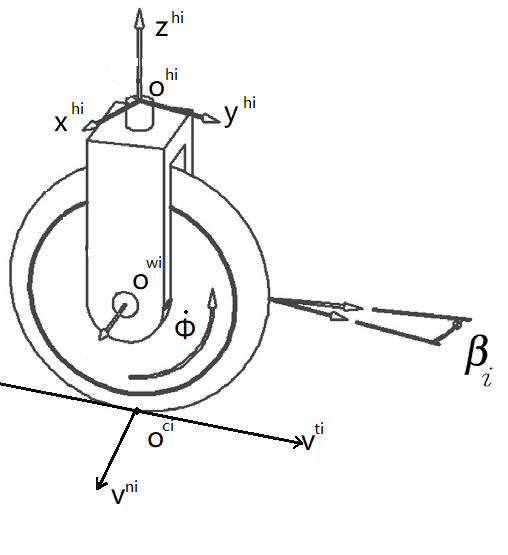
\includegraphics[width=0.8\linewidth]{Figure/wheel.png}
                    \caption{Joint configuration}
                    \label{fig:sub1}
                \end{subfigure}\hskip 1em%
                \begin{subfigure}[t]{0.5\textwidth}
                    \centering
                    \resizebox{5cm}{!}
                    {
		                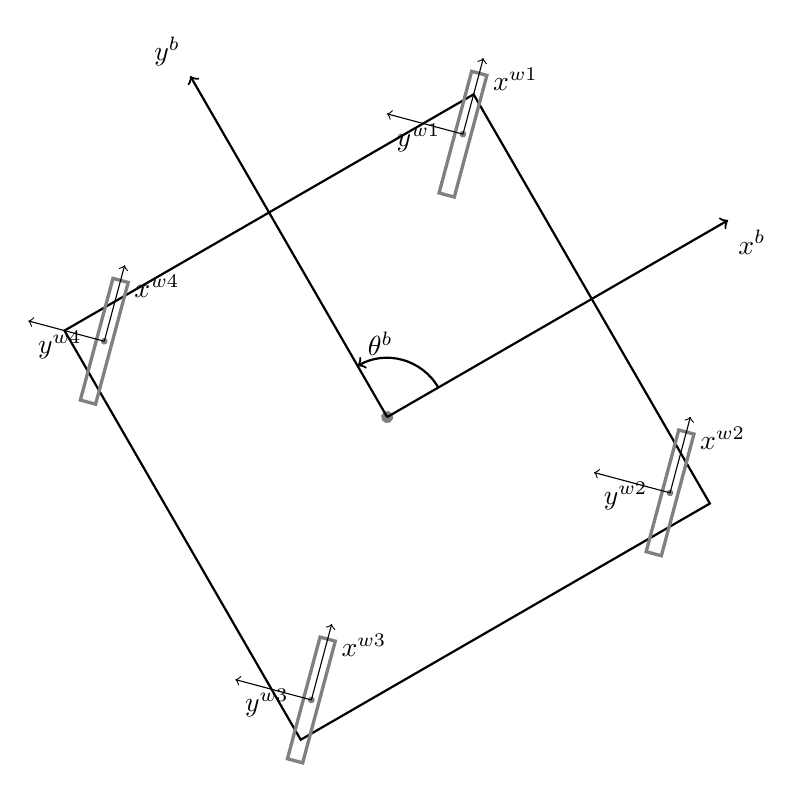
\begin{tikzpicture}[rotate=30 ]
			                \pic[rotate=30 ] at(0,0) {platform};
			                \pic[rotate=75 ] at(2.63,2.63) {wheelFrame={1}};
			                \pic[rotate=75 ] at(2.63,-2.63) {wheelFrame={2}};
			                \pic[rotate=75 ] at(-2.63,2.63) {wheelFrame={4}};
			                \pic[rotate=75 ] at(-2.63,-2.63) {wheelFrame={3}};
			                
		                \end{tikzpicture}
		            }
                    \caption{Task space velocity}
                    \label{fig:sub2}
                \end{subfigure}
            \end{figure}

\end{frame}


%%%%%%%%%%%%%%%%%%%%%%%%%%%%%%%%%%%%%%%%%%%%%%%%%%%%%%%%%%%%%%%%%
\begin{frame}{Kinematics Constraints}
    Basically there is only one kinematic constraint:\\\textbf{The wheel drives without slipping or lateral skidding}\\
    Which means the wheel contact point with ground has 0 tangential and normal velocity. $v_{ti}=0, v_{ni}=0$
    \begin{figure}
        \centering
        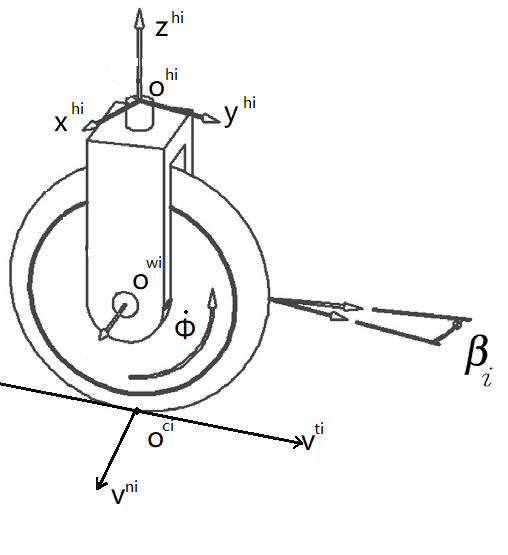
\includegraphics[width=0.5\textwidth]{Figure/wheel.png}
        \label{fig:wheel}
    \end{figure}
\end{frame}
%%%%%%%%%%%%%%%%%%%%%%%%%%%%%%%%%%%%%%%%%%%%%%%%%%%%%%%%%%%%%%%%%



%%%%%%%%%%%%%%%%%%%%%%%%%%%%%%%%%%%%%%%%%%%%%%%%%%%%%%%%%%%%%%%%%
\begin{frame}{Kinematics Constraints}
    From the $v_{ti}=0, v_{ni}=0$ constraint we can derive equations: 
    \begin{equation}\label{eq:2}
	\begin{split}
	\beta_i &= tan^{-1}(\frac{\dot{y^b}+h_{xi}\dot{\theta^b}}{\dot{x^b}-h_{yi}\dot{\theta^b}})
	\end{split}
\end{equation}

\begin{equation}\label{eq:3}
	\begin{split}
	\dot{\beta_i} &= \frac{-g(\dot{\beta_i})\ddot{\xi}}{\frac{dg(\dot{\beta_i})}{d\beta_i}\dot{\xi}}=\frac{\partial\beta_i}{\partial\dot{x}^b}\ddot{x}^b+\frac{\partial\beta_i}{\partial\dot{y}^b}\ddot{y}^b +\frac{\partial\beta_i}{\partial\dot{\theta^b}}\ddot{\theta}^b
	=f_{1i}(\dot{\xi^b})\ddot{\xi^b}
	\end{split}
\end{equation}

\begin{equation}\label{eq:4}
	\begin{split}
	\dot{\phi_i} &= \frac{1}{r_w}[cos(\beta_i), sin(\beta_i), -h_{yi}cos(\beta_i)+h_{xi}sin(\beta_i)]\dot{\xi^b}=f_{2i}(\beta)\dot{\xi^b}
	\end{split}
\end{equation}

These equations combined are called inverse kinematics(IK). Given task space command $\dot{\xi}=[\dot{x},\dot{y},\dot{\theta}]$ and $\ddot{\xi}=[\ddot{x},\ddot{y},\ddot{\theta}]$. We can use the IK to get the corresponding steering angle $\beta$, steering velocity $\dot{\beta}$ and driving speed $\dot{\phi}$
\end{frame}
%%%%%%%%%%%%%%%%%%%%%%%%%%%%%%%%%%%%%%%%%%%%%%%%%%%%%%%%%%%%%%%%%
\begin{frame}{Instantaneous center of rotation (ICR)}
    Another interpretation for the kinematics is that, if the \textbf{no slipping or lateral skidding} constraint is met. Then at each instant the motion of the robot can be viewed as an instantaneous rotation around the ICR
    \begin{figure}
	\begin{center}
	\resizebox{4cm}{!}
    {
		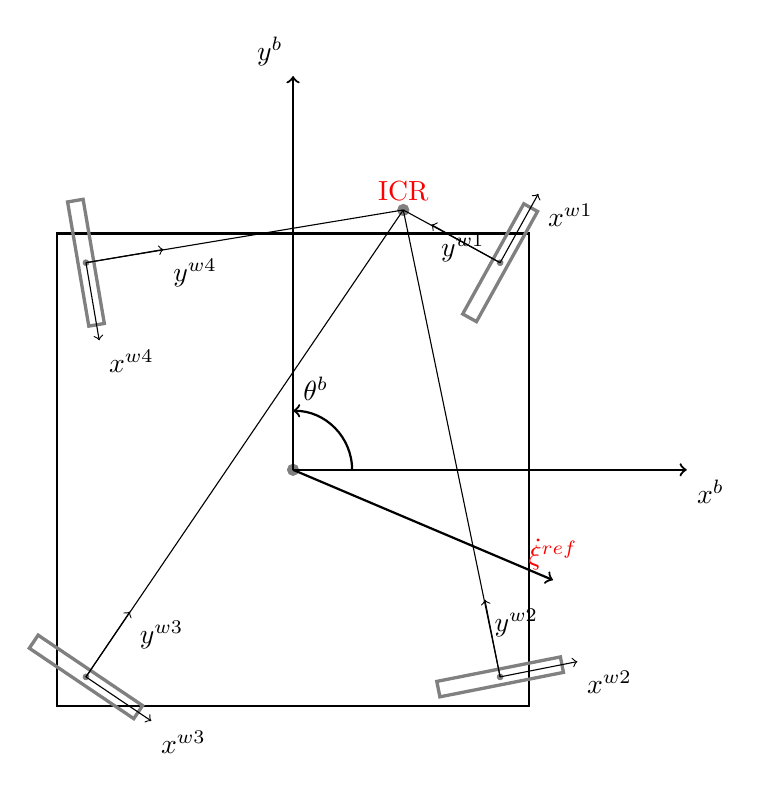
\begin{tikzpicture}
			\pic at(0,0) {platform};
			\pic[rotate=61] at(2.63,2.63) {wheelFrame={1}};
			\pic[rotate=11.2] at(2.63,-2.63) {wheelFrame={2}};
			\pic[rotate=-80.3] at(-2.63,2.63) {wheelFrame={4}};
			\pic[rotate=-34] at(-2.63,-2.63) {wheelFrame={3}};		
			\filldraw [gray] (1.4,3.3) circle (2pt) node[above,text=red]{ICR};
			\draw [rotate=-90, thick, ->] (0,0) -- (1.4,3.3) node[above,text=red]{$\dot{\xi}^{ref}$};
			\draw (2.63,2.63) -- (1.4,3.3);
			\draw (2.63,-2.63) -- (1.4,3.3);
			\draw (-2.63,-2.63) -- (1.4,3.3);
			\draw (-2.63,2.63) -- (1.4,3.3);
		\end{tikzpicture}
		}
	\end{center}
	\caption{Instantaneous Center of Rotation}
\end{figure}
Conclusion: At each time instant, the y axles of all the wheels are concurrent at the ICR.
\end{frame}

%%%%%%%%%%%%%%%%%%%%%%%%%%%%%%%%%%%%%%%%%%%%%%%%%%%%%%%%%%%%%%%%%
\section{Problem Identification}
%%%%%%%%%%%%%%%%%%%%%%%%%%%%%%%%%%%%%%%%%%%%%%%%%%%%%%%%%%%%%%%%%

\begin{frame}{Inconsistency}
    In cases like obstacle avoidance, inconsistent task space command could happen. Huge acceleration on steering is required to conduct this sudden change in 1 control cycle (0.002s).
    The wheel motor will be broken/locked\\
    e.g. Pedestrian avoiding\\
    \begin{equation}
        \dot{\xi}^n=[1,0,0] - > \dot{\xi}^{n+1}=[0,1,0]
    \end{equation}
    
   
\end{frame}
%%%%%%%%%%%%%%%%%%%%%%%%%%%%%%%%%%%%%%%%%%%%%%%%%%%%%%%%%%%%%%%%%
\begin{frame}{Inconsistency}
 \begin{figure}
	\begin{center}
	\resizebox{4cm}{!}
    {
		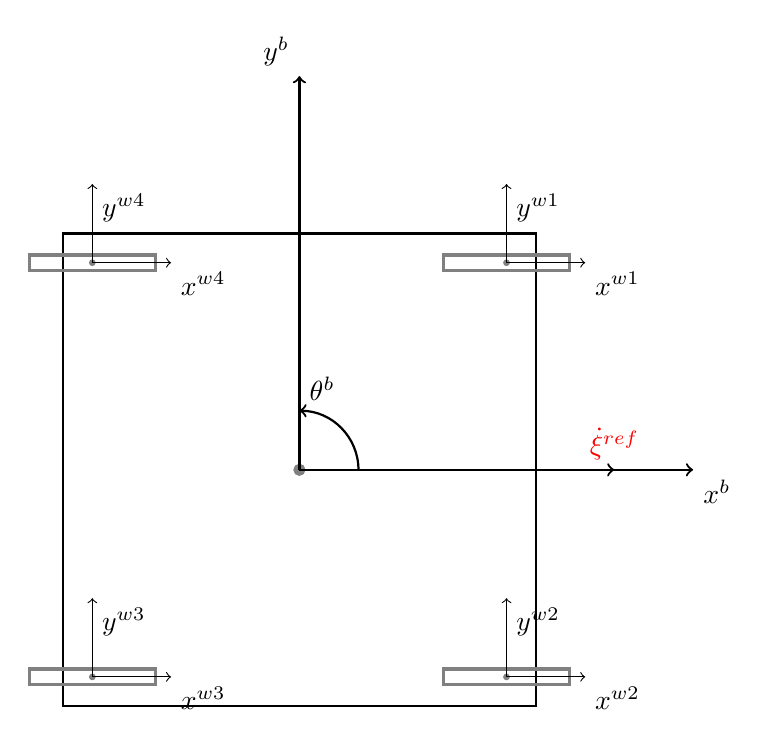
\begin{tikzpicture}
			\pic at(0,0) {platform};
			\pic[rotate=0] at(2.63,2.63) {wheelFrame={1}};
			\pic[rotate=0] at(2.63,-2.63) {wheelFrame={2}};
			\pic[rotate=0] at(-2.63,2.63) {wheelFrame={4}};
			\pic[rotate=0] at(-2.63,-2.63) {wheelFrame={3}};		
			%\filldraw [gray] (1.4,3.3) circle (2pt) node[above,text=red]{ICR};
			\draw [rotate=0, thick, ->] (0,0) -- (4,0) node[above,text=red]{$\dot{\xi}^{ref}$};
% 			\draw (2.63,2.63) -- (1.4,3.3);
% 			\draw (2.63,-2.63) -- (1.4,3.3);
% 			\draw (-2.63,-2.63) -- (1.4,3.3);
% 			\draw (-2.63,2.63) -- (1.4,3.3);
		\end{tikzpicture}
		}
	\end{center}
	\caption{$\dot{\xi}^n=[1,0,0]$}
\end{figure}
\end{frame}
%%%%%%%%%%%%%%%%%%%%%%%%%%%%%%%%%%%%%%%%%%%%%%%%%%%%%%%%%%%%%%%%%
\begin{frame}{Inconsistency}
 \begin{figure}
	\begin{center}
	\resizebox{4cm}{!}
    {
		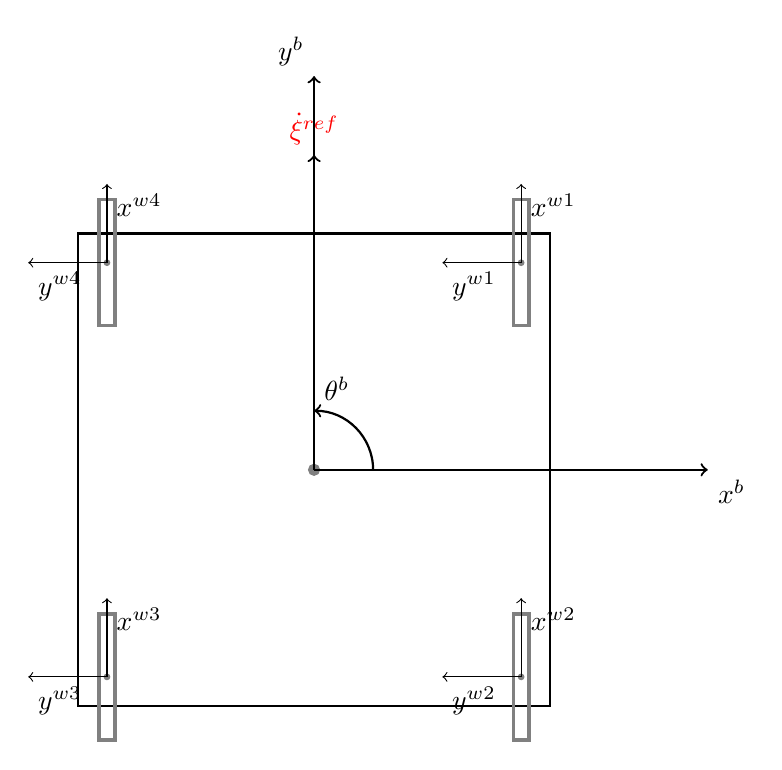
\begin{tikzpicture}
			\pic at(0,0) {platform};
			\pic[rotate=90] at(2.63,2.63) {wheelFrame={1}};
			\pic[rotate=90] at(2.63,-2.63) {wheelFrame={2}};
			\pic[rotate=90] at(-2.63,2.63) {wheelFrame={4}};
			\pic[rotate=90] at(-2.63,-2.63) {wheelFrame={3}};		
			%\filldraw [gray] (1.4,3.3) circle (2pt) node[above,text=red]{ICR};
			\draw [rotate=90, thick, ->] (0,0) -- (4,0) node[above,text=red]{$\dot{\xi}^{ref}$};
% 			\draw (2.63,2.63) -- (1.4,3.3);
% 			\draw (2.63,-2.63) -- (1.4,3.3);
% 			\draw (-2.63,-2.63) -- (1.4,3.3);
% 			\draw (-2.63,2.63) -- (1.4,3.3);
		\end{tikzpicture}
		}
	\end{center}
	\caption{$\dot{\xi}^n=[0,1,0]$}
\end{figure}
\end{frame}

%%%%%%%%%%%%%%%%%%%%%%%%%%%%%%%%%%%%%%%%%%%%%%%%%%%%%%%%%%%%%%%%%
\begin{frame}{Inconsistency}
    We can also apply the ICR interpretation on the inconsistency problem. \\
    \textbf{Inconsistency task space command corresponding to a huge change of ICR position}\\
    e.g.:
    \begin{equation}
        \dot{\xi}^n=[3.3,-1.4,1] - > \dot{\xi}^{n+1}=[0,0,1]
    \end{equation}
\end{frame}

%%%%%%%%%%%%%%%%%%%%%%%%%%%%%%%%%%%%%%%%%%%%%%%%%%%%%%%%%%%%%%%%%
\begin{frame}{Inconsistency}
     \begin{figure}
	\begin{center}
	\resizebox{4cm}{!}
    {
		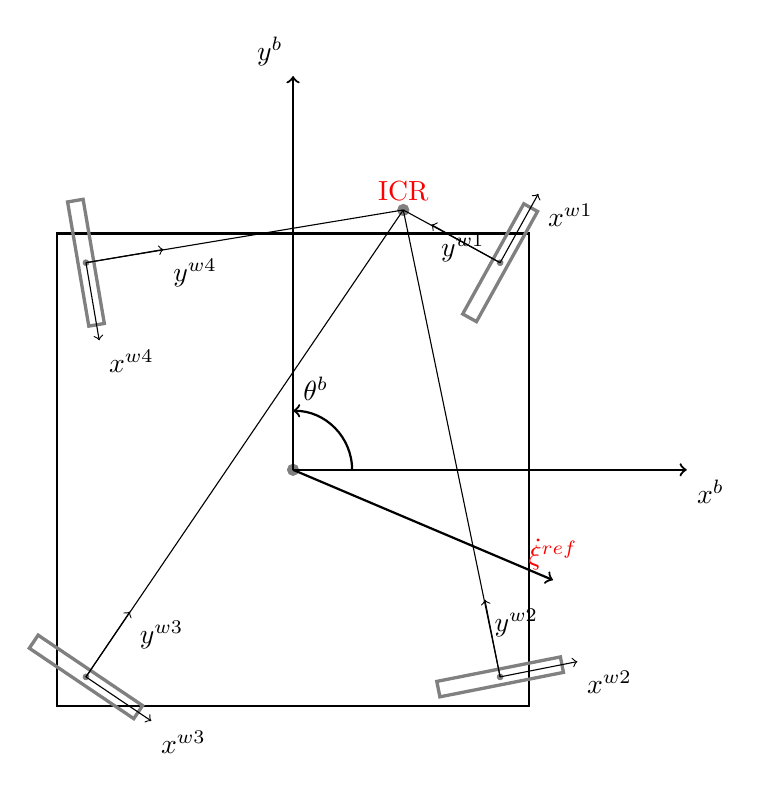
\begin{tikzpicture}
			\pic at(0,0) {platform};
			\pic[rotate=61] at(2.63,2.63) {wheelFrame={1}};
			\pic[rotate=11.2] at(2.63,-2.63) {wheelFrame={2}};
			\pic[rotate=-80.3] at(-2.63,2.63) {wheelFrame={4}};
			\pic[rotate=-34] at(-2.63,-2.63) {wheelFrame={3}};		
			\filldraw [gray] (1.4,3.3) circle (2pt) node[above,text=red]{ICR};
			\draw [rotate=-90, thick, ->] (0,0) -- (1.4,3.3) node[above,text=red]{$\dot{\xi}^{ref}$};
			\draw (2.63,2.63) -- (1.4,3.3);
			\draw (2.63,-2.63) -- (1.4,3.3);
			\draw (-2.63,-2.63) -- (1.4,3.3);
			\draw (-2.63,2.63) -- (1.4,3.3);
		\end{tikzpicture}
		}
	\end{center}
	\caption{$\dot{\xi}^n=[3.3,-1.4,1]$}
\end{figure}
\end{frame}


%%%%%%%%%%%%%%%%%%%%%%%%%%%%%%%%%%%%%%%%%%%%%%%%%%%%%%%%%%%%%%%%%

\begin{frame}{Inconsistency}
     \begin{figure}
	\begin{center}
	\resizebox{4cm}{!}
    {
		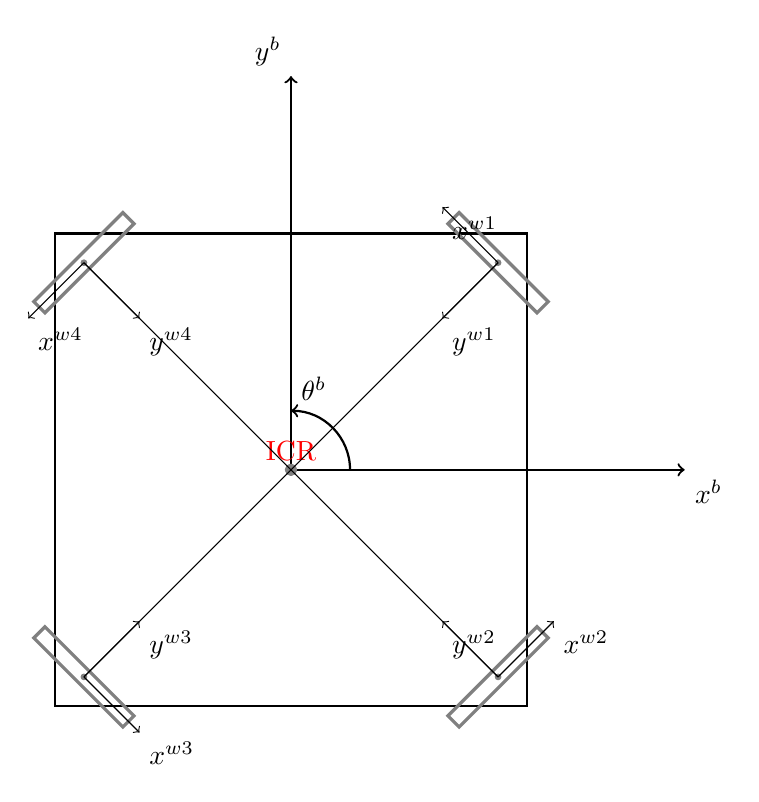
\begin{tikzpicture}
			\pic at(0,0) {platform};
			\pic[rotate=135] at(2.63,2.63) {wheelFrame={1}};
			\pic[rotate=45] at(2.63,-2.63) {wheelFrame={2}};
			\pic[rotate=-135] at(-2.63,2.63) {wheelFrame={4}};
			\pic[rotate=-45] at(-2.63,-2.63) {wheelFrame={3}};		
			\filldraw [gray] (0,0) circle (2pt) node[above,text=red]{ICR};
			%\draw [rotate=-90, thick, ->] (0,0) -- (1.4,3.3) node[above,text=red]{$\dot{\xi}^{ref}$};
			\draw (2.63,2.63) -- (0,0);
			\draw (2.63,-2.63) -- (0,0);
			\draw (-2.63,-2.63) -- (0,0);
			\draw (-2.63,2.63) -- (0,0);
		\end{tikzpicture}
		}
	\end{center}
	\caption{$\dot{\xi}^{n+1}=[0,0,1]$}
\end{figure}
\end{frame}
%%%%%%%%%%%%%%%%%%%%%%%%%%%%%%%%%%%%%%%%%%%%%%%%%%%%%%%%%%%%%%%%%
\begin{frame}[fragile]{Metropolis}

  The \themename theme is a Beamer theme with minimal visual noise
  inspired by the \href{https://github.com/hsrmbeamertheme/hsrmbeamertheme}{\textsc{hsrm} Beamer
  Theme} by Benjamin Weiss.

  Enable the theme by loading

  \begin{verbatim}    \documentclass{beamer}
    \usetheme{metropolis}\end{verbatim}

  Note, that you have to have Mozilla's \emph{Fira Sans} font and XeTeX
  installed to enjoy this wonderful typography.
\end{frame}
\begin{frame}[fragile]{Sections}
  Sections group slides of the same topic

  \begin{verbatim}    \section{Elements}\end{verbatim}

  for which \themename provides a nice progress indicator \ldots
\end{frame}

\section{Title formats}

\begin{frame}{Metropolis title formats}
	\themename supports 4 different title formats:
	\begin{itemize}
		\item Regular
		\item \textsc{Small caps}
		\item \textsc{all small caps}
		\item ALL CAPS
	\end{itemize}
	They can either be set at once for every title type or individually.
\end{frame}

{
    \metroset{titleformat frame=smallcaps}
\begin{frame}{Small caps}
	This frame uses the \texttt{smallcaps} title format.

	\begin{alertblock}{Potential Problems}
		Be aware that not every font supports small caps. If for example you typeset your presentation with pdfTeX and the Computer Modern Sans Serif font, every text in small caps will be typeset with the Computer Modern Serif font instead.
	\end{alertblock}
\end{frame}
}

{
\metroset{titleformat frame=allsmallcaps}
\begin{frame}{All small caps}
	This frame uses the \texttt{allsmallcaps} title format.

	\begin{alertblock}{Potential problems}
		As this title format also uses small caps you face the same problems as with the \texttt{smallcaps} title format. Additionally this format can cause some other problems. Please refer to the documentation if you consider using it.

		As a rule of thumb: just use it for plaintext-only titles.
	\end{alertblock}
\end{frame}
}

{
\metroset{titleformat frame=allcaps}
\begin{frame}{All caps}
	This frame uses the \texttt{allcaps} title format.

	\begin{alertblock}{Potential Problems}
		This title format is not as problematic as the \texttt{allsmallcaps} format, but basically suffers from the same deficiencies. So please have a look at the documentation if you want to use it.
	\end{alertblock}
\end{frame}
}

\section{Elements}

\begin{frame}[fragile]{Typography}
      \begin{verbatim}The theme provides sensible defaults to
\emph{emphasize} text, \alert{accent} parts
or show \textbf{bold} results.\end{verbatim}

  \begin{center}becomes\end{center}

  The theme provides sensible defaults to \emph{emphasize} text,
  \alert{accent} parts or show \textbf{bold} results.
\end{frame}

\begin{frame}{Font feature test}
  \begin{itemize}
    \item Regular
    \item \textit{Italic}
    \item \textsc{Small Caps}
    \item \textbf{Bold}
    \item \textbf{\textit{Bold Italic}}
    \item \textbf{\textsc{Bold Small Caps}}
    \item \texttt{Monospace}
    \item \texttt{\textit{Monospace Italic}}
    \item \texttt{\textbf{Monospace Bold}}
    \item \texttt{\textbf{\textit{Monospace Bold Italic}}}
  \end{itemize}
\end{frame}

\begin{frame}{Lists}
  \begin{columns}[T,onlytextwidth]
    \column{0.33\textwidth}
      Items
      \begin{itemize}
        \item Milk \item Eggs \item Potatoes
      \end{itemize}

    \column{0.33\textwidth}
      Enumerations
      \begin{enumerate}
        \item First, \item Second and \item Last.
      \end{enumerate}

    \column{0.33\textwidth}
      Descriptions
      \begin{description}
        \item[PowerPoint] Meeh. \item[Beamer] Yeeeha.
      \end{description}
  \end{columns}
\end{frame}
\begin{frame}{Animation}
  \begin{itemize}[<+- | alert@+>]
    \item \alert<4>{This is\only<4>{ really} important}
    \item Now this
    \item And now this
  \end{itemize}
\end{frame}
\begin{frame}{Figures}
  \begin{figure}
    \newcounter{density}
    \setcounter{density}{20}
    \begin{tikzpicture}
      \def\couleur{alerted text.fg}
      \path[coordinate] (0,0)  coordinate(A)
                  ++( 90:5cm) coordinate(B)
                  ++(0:5cm) coordinate(C)
                  ++(-90:5cm) coordinate(D);
      \draw[fill=\couleur!\thedensity] (A) -- (B) -- (C) --(D) -- cycle;
      \foreach \x in {1,...,40}{%
          \pgfmathsetcounter{density}{\thedensity+20}
          \setcounter{density}{\thedensity}
          \path[coordinate] coordinate(X) at (A){};
          \path[coordinate] (A) -- (B) coordinate[pos=.10](A)
                              -- (C) coordinate[pos=.10](B)
                              -- (D) coordinate[pos=.10](C)
                              -- (X) coordinate[pos=.10](D);
          \draw[fill=\couleur!\thedensity] (A)--(B)--(C)-- (D) -- cycle;
      }
    \end{tikzpicture}
    \caption{Rotated square from
    \href{http://www.texample.net/tikz/examples/rotated-polygons/}{texample.net}.}
  \end{figure}
\end{frame}
\begin{frame}{Tables}
  \begin{table}
    \caption{Largest cities in the world (source: Wikipedia)}
    \begin{tabular}{@{} lr @{}}
      \toprule
      City & Population\\
      \midrule
      Mexico City & 20,116,842\\
      Shanghai & 19,210,000\\
      Peking & 15,796,450\\
      Istanbul & 14,160,467\\
      \bottomrule
    \end{tabular}
  \end{table}
\end{frame}
\begin{frame}{Blocks}
  Three different block environments are pre-defined and may be styled with an
  optional background color.

  \begin{columns}[T,onlytextwidth]
    \column{0.5\textwidth}
      \begin{block}{Default}
        Block content.
      \end{block}

      \begin{alertblock}{Alert}
        Block content.
      \end{alertblock}

      \begin{exampleblock}{Example}
        Block content.
      \end{exampleblock}

    \column{0.5\textwidth}

      \metroset{block=fill}

      \begin{block}{Default}
        Block content.
      \end{block}

      \begin{alertblock}{Alert}
        Block content.
      \end{alertblock}

      \begin{exampleblock}{Example}
        Block content.
      \end{exampleblock}

  \end{columns}
\end{frame}
\begin{frame}{Math}
  \begin{equation*}
    e = \lim_{n\to \infty} \left(1 + \frac{1}{n}\right)^n
  \end{equation*}
\end{frame}
\begin{frame}{Line plots}
  \begin{figure}
    \begin{tikzpicture}
      \begin{axis}[
        mlineplot,
        width=0.9\textwidth,
        height=6cm,
      ]

        \addplot {sin(deg(x))};
        \addplot+[samples=100] {sin(deg(2*x))};

      \end{axis}
    \end{tikzpicture}
  \end{figure}
\end{frame}
\begin{frame}{Bar charts}
  \begin{figure}
    \begin{tikzpicture}
      \begin{axis}[
        mbarplot,
        xlabel={Foo},
        ylabel={Bar},
        width=0.9\textwidth,
        height=6cm,
      ]

      \addplot plot coordinates {(1, 20) (2, 25) (3, 22.4) (4, 12.4)};
      \addplot plot coordinates {(1, 18) (2, 24) (3, 23.5) (4, 13.2)};
      \addplot plot coordinates {(1, 10) (2, 19) (3, 25) (4, 15.2)};

      \legend{lorem, ipsum, dolor}

      \end{axis}
    \end{tikzpicture}
  \end{figure}
\end{frame}
\begin{frame}{Quotes}
  \begin{quote}
    Veni, Vidi, Vici
  \end{quote}
\end{frame}

{%
\setbeamertemplate{frame footer}{My custom footer}
\begin{frame}[fragile]{Frame footer}
    \themename defines a custom beamer template to add a text to the footer. It can be set via
    \begin{verbatim}\setbeamertemplate{frame footer}{My custom footer}\end{verbatim}
\end{frame}
}

\begin{frame}{References}
  Some references to showcase [allowframebreaks] \cite{knuth92,ConcreteMath,Simpson,Er01,greenwade93}
\end{frame}

\section{Conclusion}

\begin{frame}{Summary}

  Get the source of this theme and the demo presentation from

  \begin{center}\url{github.com/matze/mtheme}\end{center}

  The theme \emph{itself} is licensed under a
  \href{http://creativecommons.org/licenses/by-sa/4.0/}{Creative Commons
  Attribution-ShareAlike 4.0 International License}.

  \begin{center}\ccbysa\end{center}

\end{frame}

\begin{frame}[standout]
  Questions?
\end{frame}

\appendix

\begin{frame}[fragile]{Backup slides}
  Sometimes, it is useful to add slides at the end of your presentation to
  refer to during audience questions.

  The best way to do this is to include the \verb|appendixnumberbeamer|
  package in your preamble and call \verb|\appendix| before your backup slides.

  \themename will automatically turn off slide numbering and progress bars for
  slides in the appendix.
\end{frame}

\begin{frame}[allowframebreaks]{References}

  \bibliography{demo}
  \bibliographystyle{abbrv}

\end{frame}

\end{document}
